
\documentclass[a4paper,12pt,french] {article}

\usepackage[sujet]{../../Style}

\fancyhead[L]{21/03/2022}
\fancyhead[C]{\textbf{DS5 : Fonctions affines et Variations de fonctions}}
\fancyhead[R]{\seconde 12}

\begin{document}

\rem{L'usage de la calculatrice est interdit. La propreté et l'orthographe seront prises en compte. Tout le devoir peut être fait sur le sujet.}

Nom: \hfill Prénom: \hfill \

\renewcommand{\baselinestretch}{1.3}

\begin{exercice}
Résoudre les équations suivantes:
\begin{center}
\begin{minipage}{0.7\textwidth}
$4x-1=8+x$ \hfill $(-2x+7)(x+1)=0$
\end{minipage}
\end{center}

\vspace{5cm}

\end{exercice}

\vfill

\begin{exercice} \

\compoligne
{
\begin{enumerate}
\item Tracer les droites $d_1$ et $d_2$ d'équations:
$$d_1:y=-3x+3,5 \ \text{ et } \ d_2:y=\frac 3 2 x-1$$
\end{enumerate}
\begin{centrer}
\begin{tikzpicture}
\begin{axis}[
styleglobal,
width=0.8*\linewidth,
xmin=-2, xmax=5,
ymin=-2, ymax=5,
xtick distance=1,
ytick distance=1,
%major grid style={line width=1pt},
]
\end{axis}
\end{tikzpicture}
\end{centrer}
}
{
\begin{enumerate}[start=2]
\item Déterminer l'équation des droites $d_3$ et $d_4$.
$$\vphantom{\frac 2 3}d_3:y=\hspace{2cm} \text{ et } d_4:y=\hspace{2cm}$$ %vphantom pour l'alignement avec la colonne de gauche
\end{enumerate}
\begin{centrer}
\begin{tikzpicture}
\begin{axis}[
styleglobal,
width=0.8*\linewidth,
xmin=-2, xmax=5,
ymin=-2, ymax=5,
xtick distance=1,
ytick distance=1,
%major grid style={line width=1pt},
]
\addplot[styleplot]{-1*x+2.5} node[pos=0.8,above right] {$d_3$};
\addplot[color=blue,styleplot,densely dotted]{3/4*x+1} node[pos=0.8,below right] {$d_4$};
\end{axis}
\end{tikzpicture}
\end{centrer}
}

\begin{enumerate}[start=3]
\item En résolvant une équation, déterminer les coordonnées du point d'intersection de $d_1$ et $d_2$.

\points 4
\end{enumerate} 
\end{exercice}

\begin{exercice}
Soit $f$ une fonction affine telle que $f(1)=1$ et $f(3)=5$. Déterminer l'expression de $f$.

\points 5

\end{exercice}

\begin{exercice}

Dresser le tableau de signes de la fonction $f:x \mapsto 5(x-3)(3x+6)$:\strut

\compo[0.4]
{
\points 6
}
{
\begin{center}
\begin{tikzpicture}
\tkzTabInit[lgt=2.5]{ /1, /4}{$- \infty$,,$+\infty$}
\end{tikzpicture}
\end{center}
}

\end{exercice}

\begin{exercice} \

\begin{enumerate}
\item Soit $f$ une fonction définie sur $[4;13]$, croissante sur $[4;6]$, décroissante sur $[6;10]$ puis croissante sur $[10;13]$. Comparer $f(11)$ et $f(12,5)$.

\points 3

\item Dresser le tableau de variations de la fonction $g$ représentée ci-contre.

\compo[0.5]
{
\begin{center}
\begin{tikzpicture}
\tkzTabInit[lgt=1.4]{ /1, /2}{,,}
\end{tikzpicture}
\end{center}
}
{
\begin{center}
\begin{tikzpicture}
\begin{axis}[
styleglobal,
width=0.9*\linewidth,
xmin=-3.5, xmax=7.5,
ymin=-2.5, ymax=3.5,
xtick distance=1,
ytick distance=1,
minor x tick num=1,
minor y tick num=1,
]
\addplot[styleplot,tension=0.3] plot coordinates{(-3,2.5) (-1,1.5) (1,-2) (3,1) (5,0.5) (6,2) (7,3)} node[pos=0.9,below right] {$\mathscr C_g$} \pointsextremites;
\end{axis}
\end{tikzpicture}
\end{center}
}

\item Quel est le minimum de $g$ sur l'intervalle $[-3;7]$? Sur l'intervalle $[3;6]$?

\points 3

\end{enumerate}
\end{exercice}

\end{document}